
    \subsection*{The problem}

        Now, our goal is to create a \textbf{good model} for our problem, \textbf{binary classification}.
        
        To do this, we can \textbf{try} using our 0-1 loss $\loss$:
        
        \begin{equation}
            J(\theta, \theta_0) = 
            \frac{1}{n} \sum_{i=1}^n 
            \loss
            (
                \red{
                    \text{sign}(\theta^T\ex{x}{i} + \theta_0)
                    }, 
                \ex{y}{i}
            )
        \end{equation}
        
        The \textbf{first} thing to note is that there isn't an easy \textbf{analytical} solution, no simple \textbf{equation}: sign$(u)$ isn't a function that we can explicitly \textbf{solve}, like we could for \textbf{linear regression}.
            \note{To be fair, this is true for most possible problems: most of them can't be solved analytically.}
            
        So, we refer to our other approach, \textbf{gradient descent}.
        
        But in order to do that, we'll just need to get the \textbf{gradient}.
        
        \begin{equation}
            \nabla_\theta J = 0
        \end{equation}
        
        ...Well that's not good.
            \note{Why not? Because we use our \textbf{gradient} to decide \textbf{how} to change $\theta$, if the gradient is 0, we'll never \textbf{improve} $\theta$ at all!}
        
    \subsection*{The real problem: sign$(u)$ is flat}
    
        What's going on here? Let's look at the sign function:
        
        \begin{figure}[H]
            \centering
            
            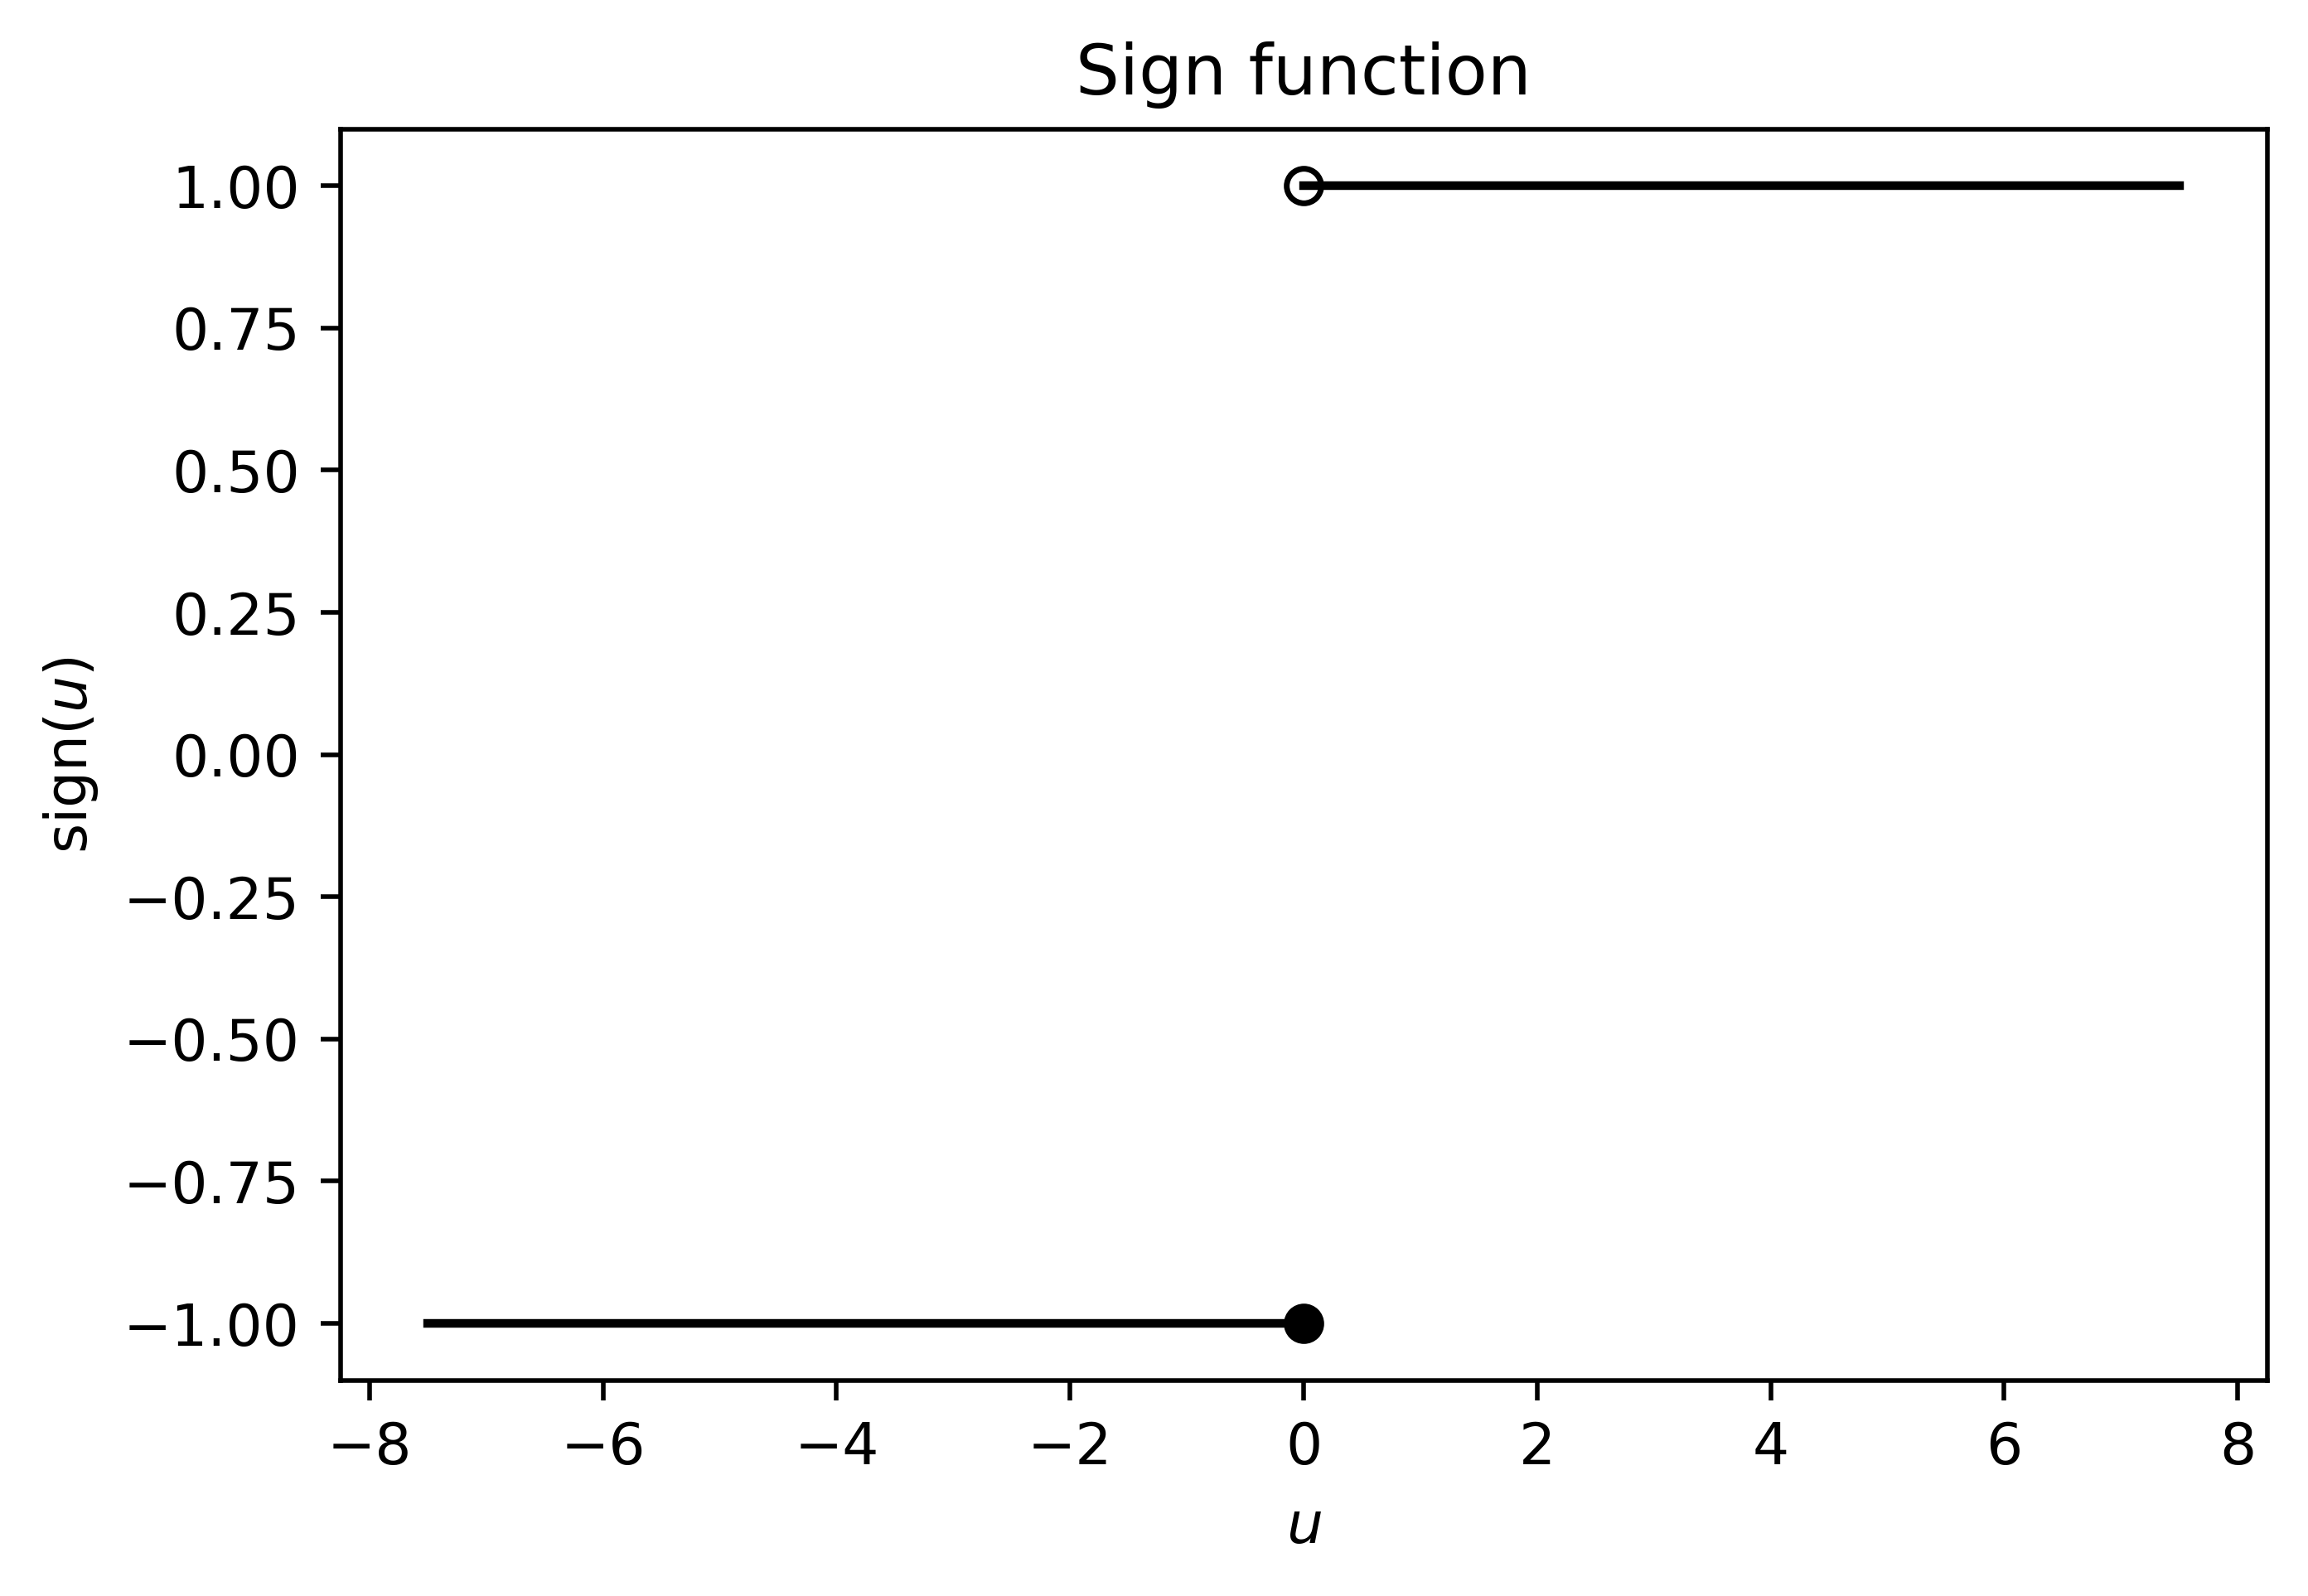
\includegraphics[width=70mm,scale=0.5]{images/classification_images/sign_function.png}
            \caption*{Sign is a flat function! The slope is 0 everywhere, except $u=0$, where it's \textbf{undefined}.}
        \end{figure}
        
        Well, that explains why we can't use the gradient: the function is \textbf{flat}.
        
        Another way to say this is that our function doesn't \textbf{tell} us when we're \textbf{closer} to being right.
        
        There's \textbf{no difference} between being \textbf{wrong} by 1 unit or being wrong by 10 units: you can't tell if you're getting \textbf{closer} to a correct answer.
        
        And the \textbf{gradient} doesn't tell you which way to move in \textbf{parameter space} to further improve.
            \note{Remember, parameter space is what we move through as we change our parameter vector $\theta$.}
        
        In fact, the best way we know how to approach this kind of problem takes \textbf{exponential} time: it takes exponentially \textbf{longer} to solve based on our \textbf{number} of data points.
        
        That's way too \textbf{slow}. So, we'll have to come up with a \textbf{better} function: something to \textbf{replace} sign$(u)$, that still serves the same role.\\
        
        \begin{concept}
            The \vocab{sign function} is difficult to optimize, because it isn't \purp{smooth}: not only is the slope undefined at 0, it is 0 everywhere else.
            
            This causes two problems:
            
            \begin{itemize}
                \item We can't tell whether one \gren{hypothesis} is \vocab{closer} to being \purp{correct}, if it has gotten \gren{better}, unless its accuracy has increased. 
                    \begin{itemize}
                        \item This makes it harder to \gren{improve}.
                    \end{itemize}
                
                \item We can't indicate how \purp{certain} we are in our answer: sign$(u)$ is \gren{all-or-nothing}: we choose one class, with no information about how \purp{confident} we are in our choice.
                    \begin{itemize}
                        \item Knowing how \purp{uncertain} we are can be \gren{helpful}, both for \gren{improving} our machine and also \gren{judging} the choices or machine makes.
                    \end{itemize}
            \end{itemize}
        \end{concept}
        
        So, we need to explore a \textbf{new} approach: we'll \textbf{replace} sign$(u)$ with something else.
    
    \subsection*{The sigmoid function}
    
        So, what do we \textbf{replace} sign with? We like the way sign \textbf{works} (choosing between two different classes based on a \textbf{threshold}), so maybe we want a \textbf{smoother} version of it.
        
        \begin{figure}[H]
            \centering
            
            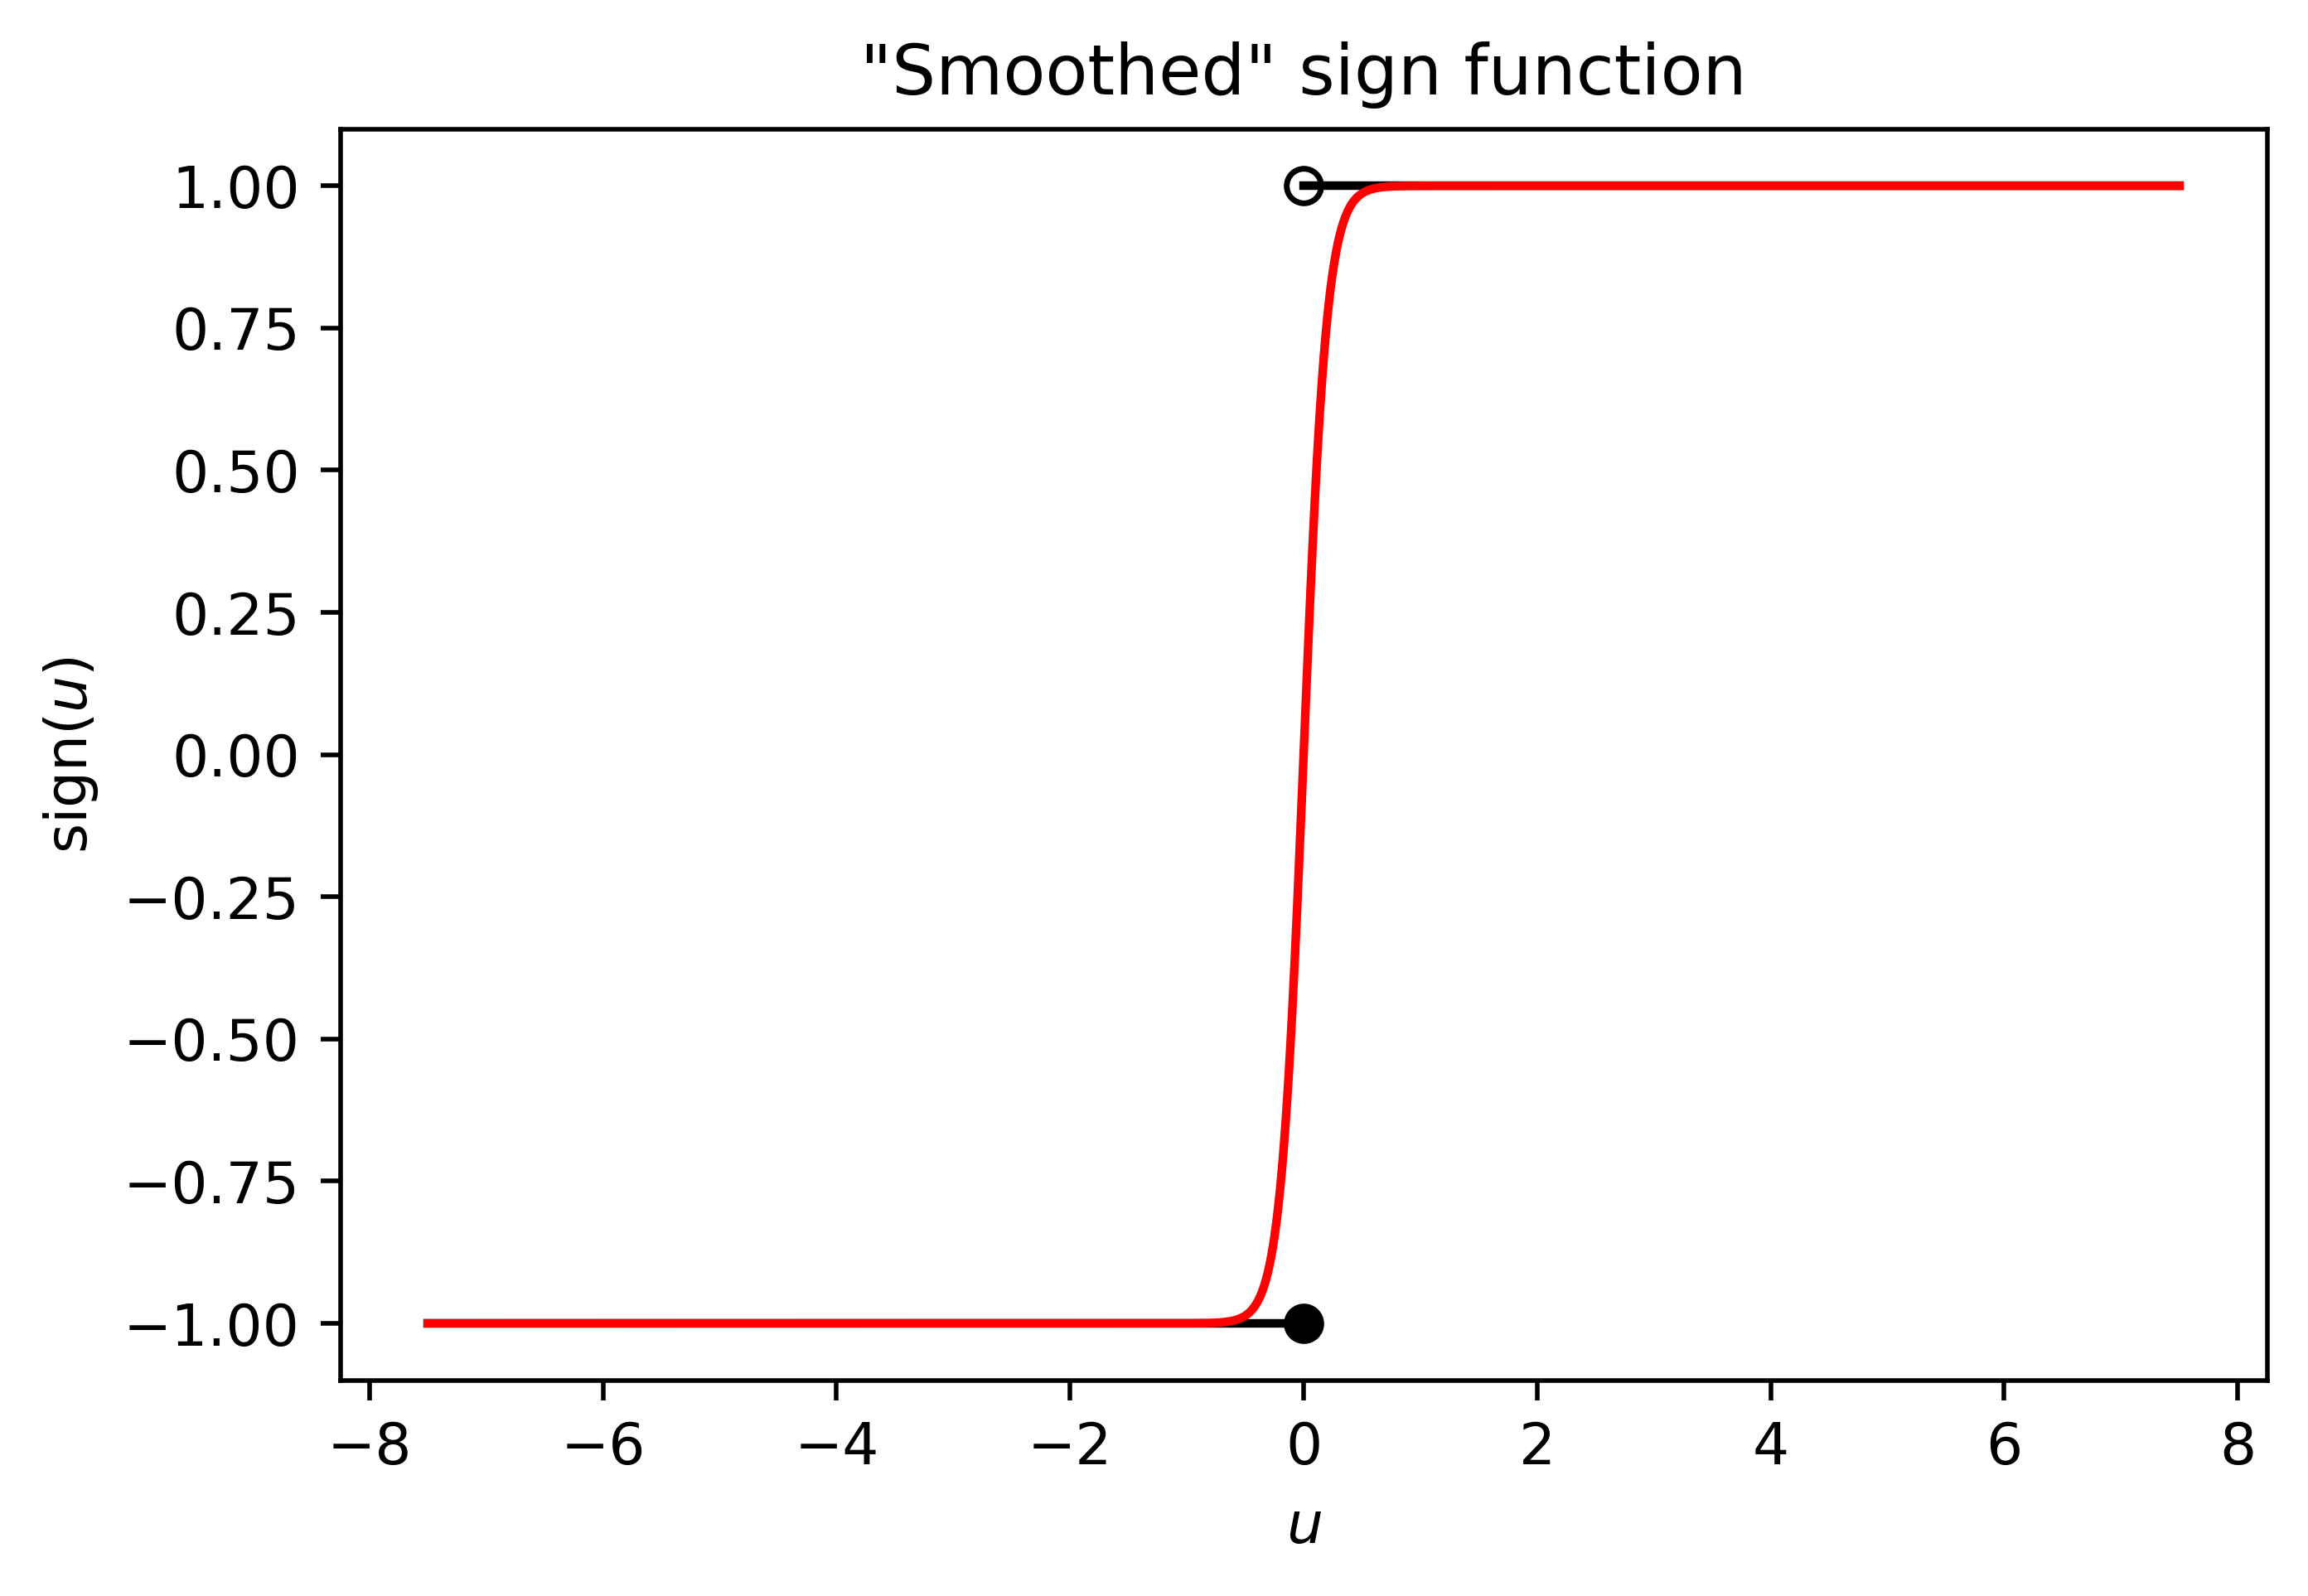
\includegraphics[width=70mm,scale=0.5]{images/classification_images/smoothed_sign_function.png}
            \caption*{The red line shows a "\textbf{smoother}" sign function, that mostly behaves the same, while solving our problem.}
        \end{figure}
        
        This solves \textbf{one} of our two problems: the \textbf{gradient} is \textbf{nonzero}. 
            \note{It's hard to see visually, but the function is \textbf{smooth}, and the slope is nonzero \textbf{everywhere}!}
        
        We could also make it less steep:
        
        \begin{figure}[H]
            \centering
            
            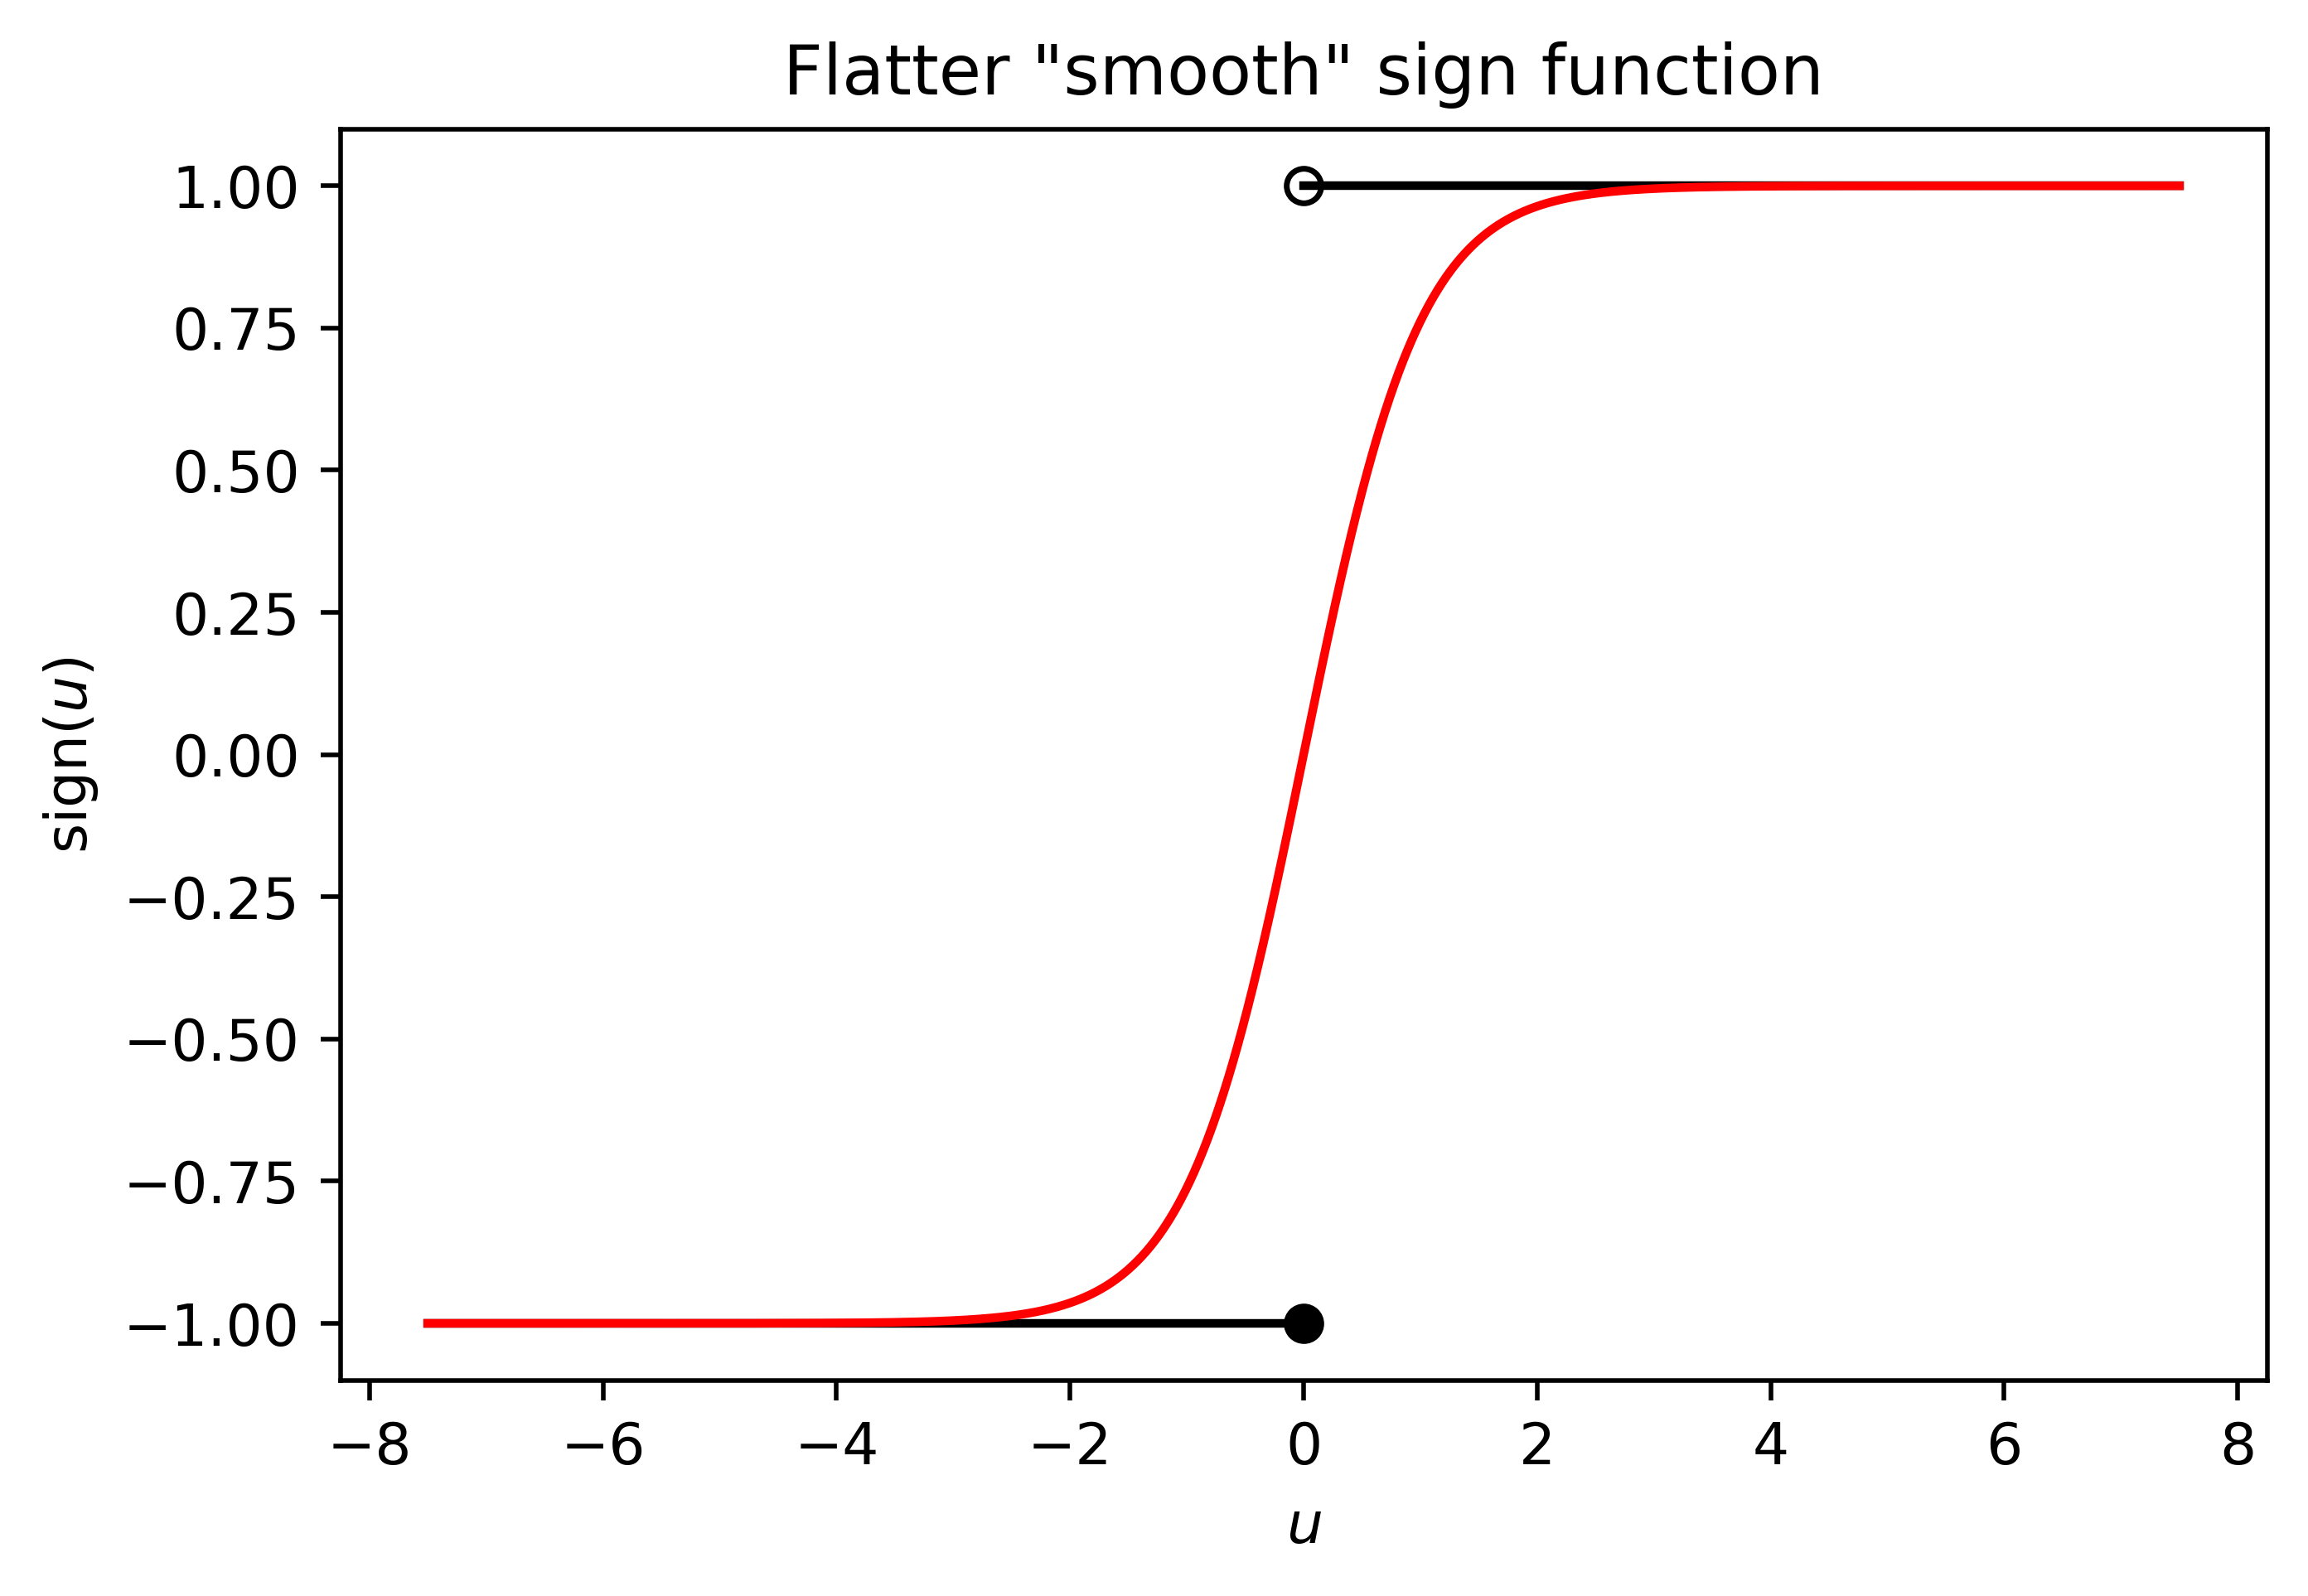
\includegraphics[width=70mm,scale=0.5]{images/classification_images/flatter_smooth_sign_function.png}
        \end{figure}
        
        So, we need a \textbf{function} that accomplishes this. It turns out there are \textbf{several} that work: $\tanh{u}$, for example.
        
        For our purposes, we'll use the following function:\\
        
        \begin{definition}
            The \vocab{sigmoid} function
            
            \begin{equation}
                \sigma(u) = \frac{1}{1+e^{-u}}
            \end{equation}
            
            ...is a \purple{nonlinear} function that we use to \gren{compute} the output of our \vocab{classification} problem.
            
            It is also called the \vocab{logistic} function.
        \end{definition}
        
        The function looks like this:
        
        \begin{figure}[H]
            \centering
            
            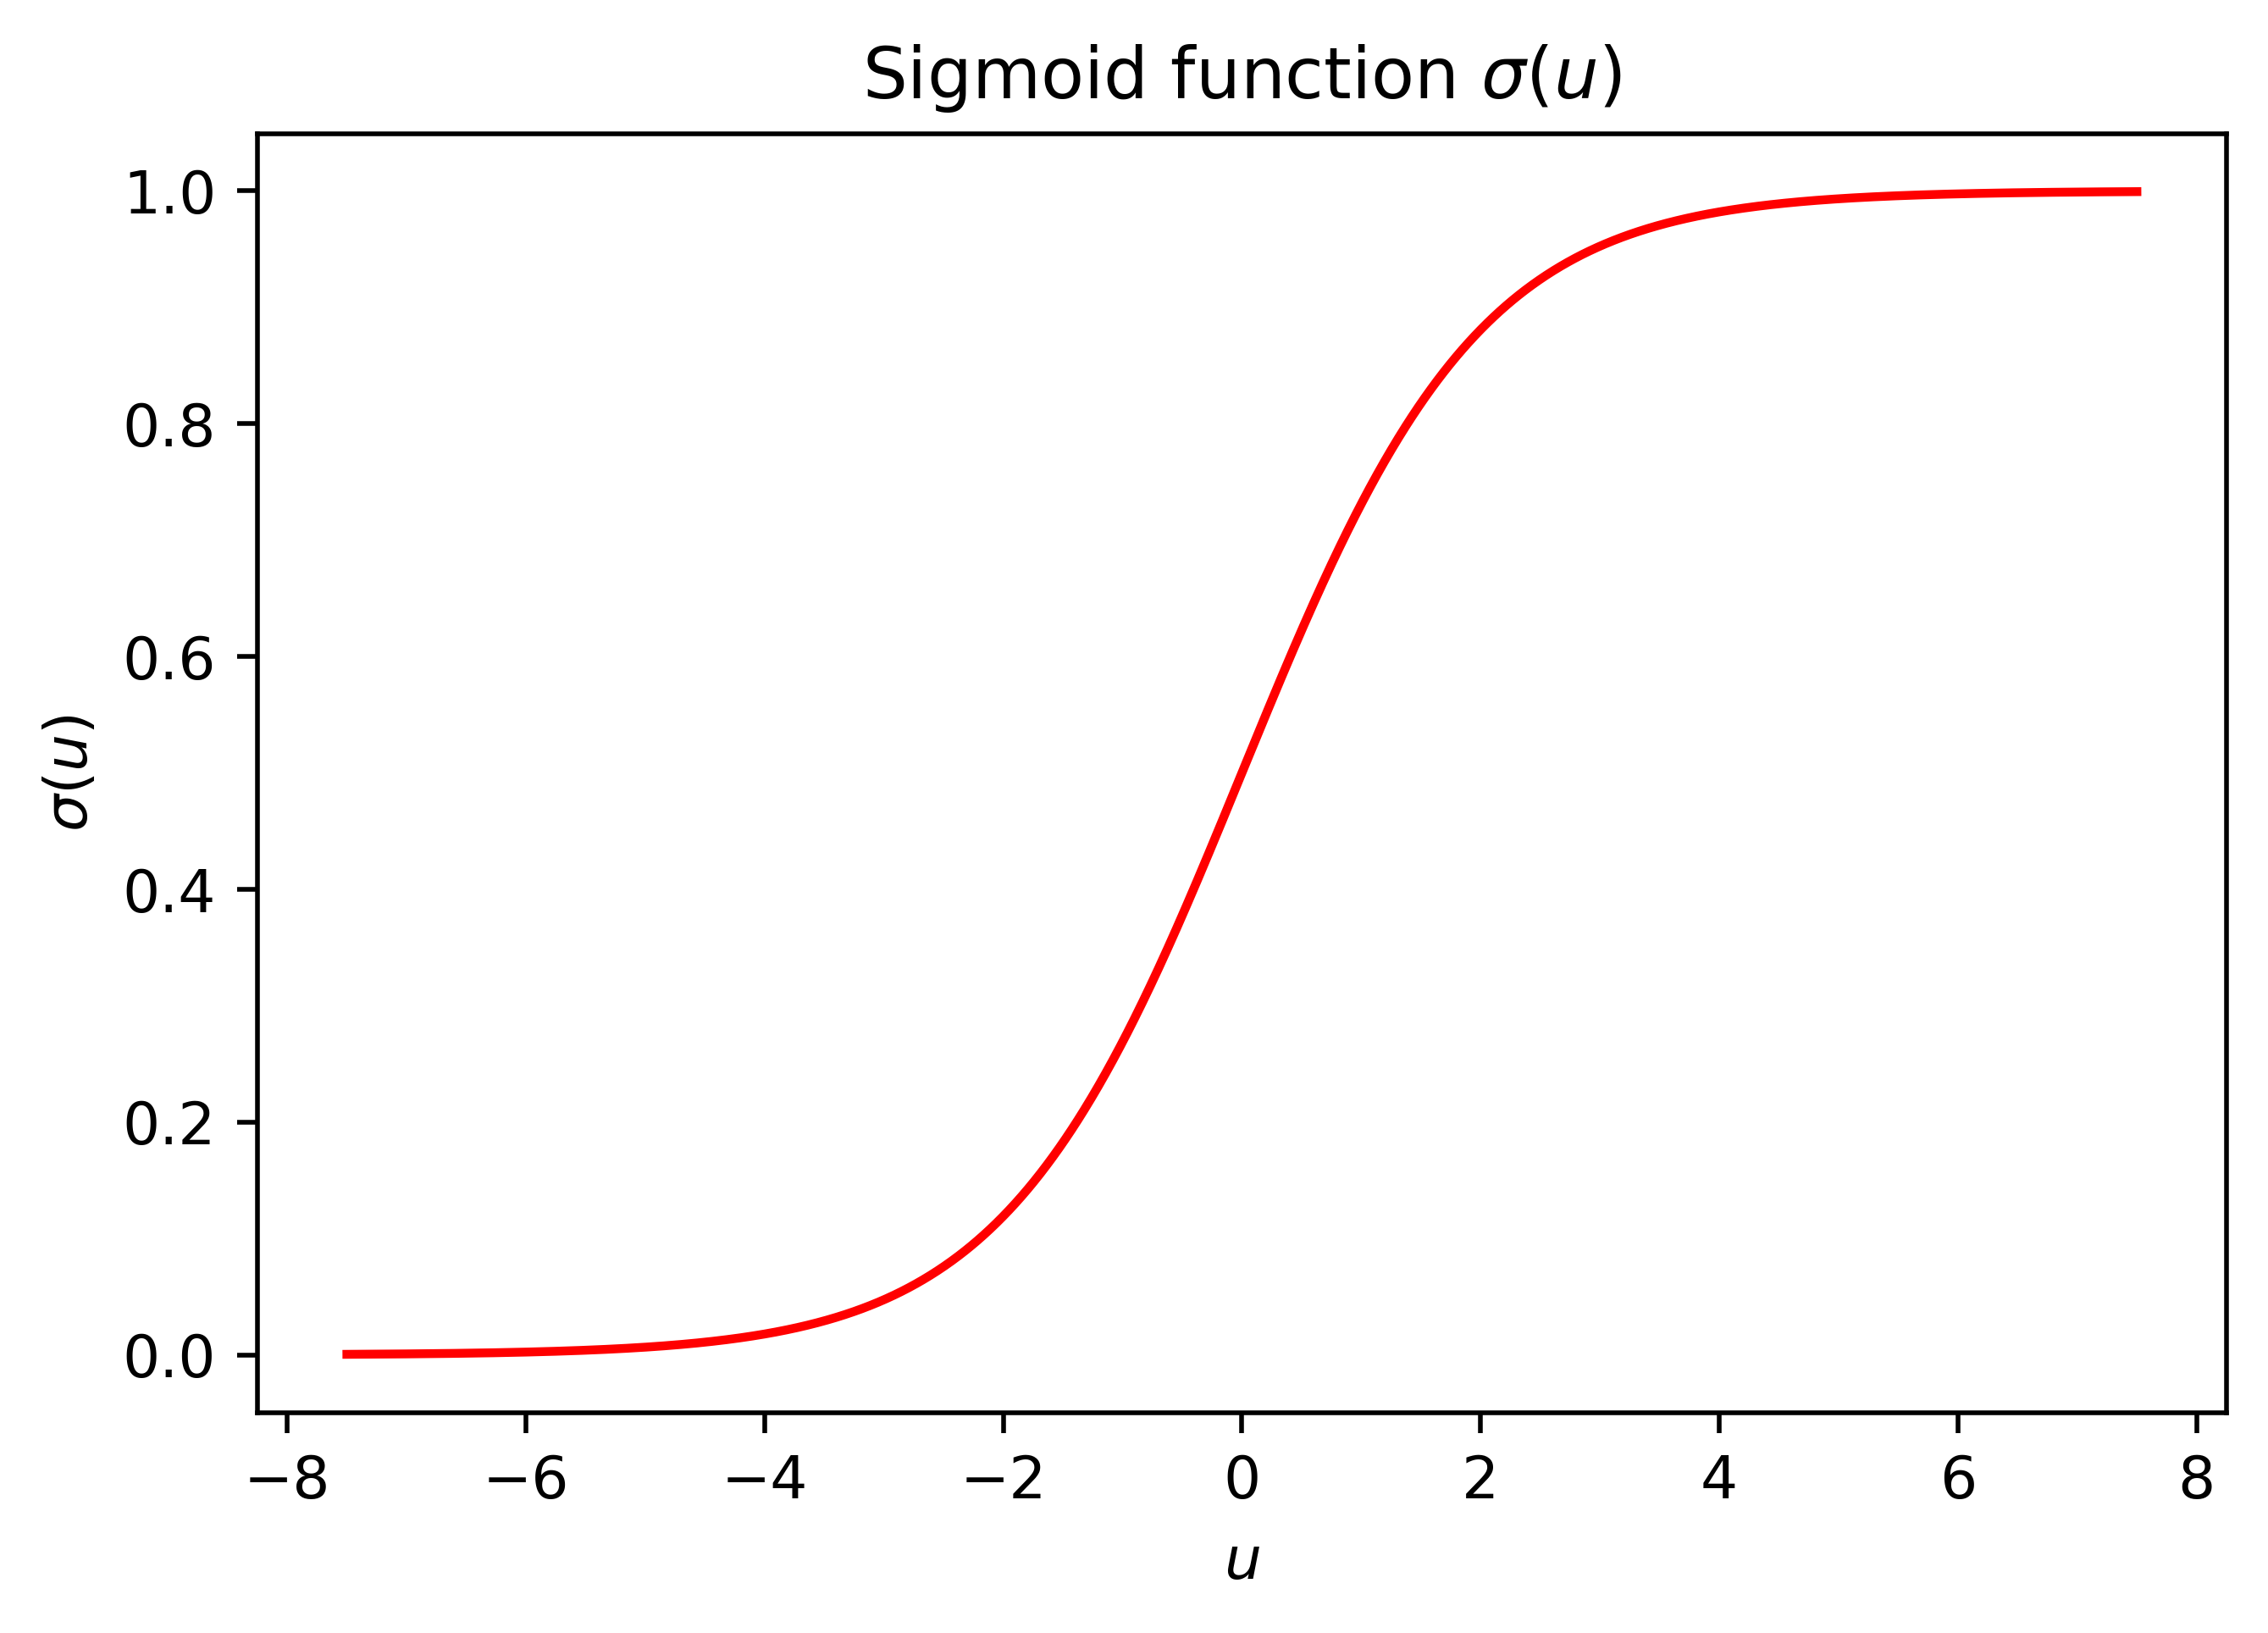
\includegraphics[width=70mm,scale=0.5]{images/classification_images/sigmoid_u.png}
        \end{figure}
        
    \subsection*{Sigmoid as a probability}
        
        Something you may \textbf{notice} is that $\sigma(x)$ is always between 0 and 1. But before, sign$(x)$ was \textbf{always} between -1 and +1. Why would we use \textit{this} function?
        
        Because going between 0 and 1 has a different advantage: we can interpret it as a \textbf{probability}.
        
        Your \textbf{value} of $\sigma(u)$ can be stated as, "what does the machine think is the \textbf{probability} we \textbf{classify} this data point as +1".
        
        And, on the \textbf{flip} side, $1-\sigma(u)$ is the \textbf{probability} we \textbf{classify} as $-1$.
        
        This solves the second problem we mentioned \textbf{earlier}: we can indicate how \textbf{confident} the machine is in its answer!\\
        
        \begin{concept}
            The output of the \vocab{sigmoid function} $\sigma(\red{u(x)})$ gives the \purp{probability} that the data point $x$ is classified \gren{positively}.
            
            \begin{equation*}
                \quad \;\; \sigma(u) = \p{ x\text{ is classified }+1 }
            \end{equation*}
            \begin{equation*}
                1 - \sigma(u) = \p{ x\text{ is classified }-1 }
            \end{equation*}
            
            Note that this works because $\sigma(u) \in (0,1)$.
        \end{concept}
        
    \subsection*{Logistic Regression}
    
        So, we've seen the benefits of switching from sign$(u)$ to $\sigma(u)$. So we'll do that:
            \note{We're using $u(x)=\theta^T x + \theta_0$}\\
        
        
        \begin{kequation}
            \vocab{Logistic Regression} is a \purp{modification} of \gren{linear regression}.
            
            \begin{equation*}
                h(x; \theta) = \sigma(\theta^T x + \theta_0 )
            \end{equation*}
        
            \centerline{where}
            
            \begin{equation*}
                \sigma(u) = \frac{1}{1+e^{-u}}
            \end{equation*}
            
            It outputs the \vocab{probability} of a \purp{positive} classification.
        \end{kequation}
        
        If we \textbf{plug} this in, we get this slightly ugly expression:
        
        \begin{equation*}
            h(x; \theta) = \frac{1}{1+e^{-(\theta^T x + \theta_0) } }
        \end{equation*}
        
        We have a problem, though: \textbf{logistic regression} is a... \vocab{regression} function. It takes in a real \textbf{vector}, and outputs a real \textbf{number}: $\RR^d \rightarrow \RR$.
        
        We can't use this to do \textbf{classification}, where want $\RR^d \rightarrow \{-1,+1\}$!
        
    \subsection*{Prediction Threshold}
    
        When we were just using $u(x) = \theta^T x + \theta_0$, we classified data points by saying whether $u(x)>0$. Our boundary was $u(x)=0$.
        
        We can't quite do that here, because $\sigma(u)=0$ is \textbf{impossible}: $\sigma(u)$ is \textbf{always} greater than 0.
        
        \begin{figure}[H]
            \centering
            
            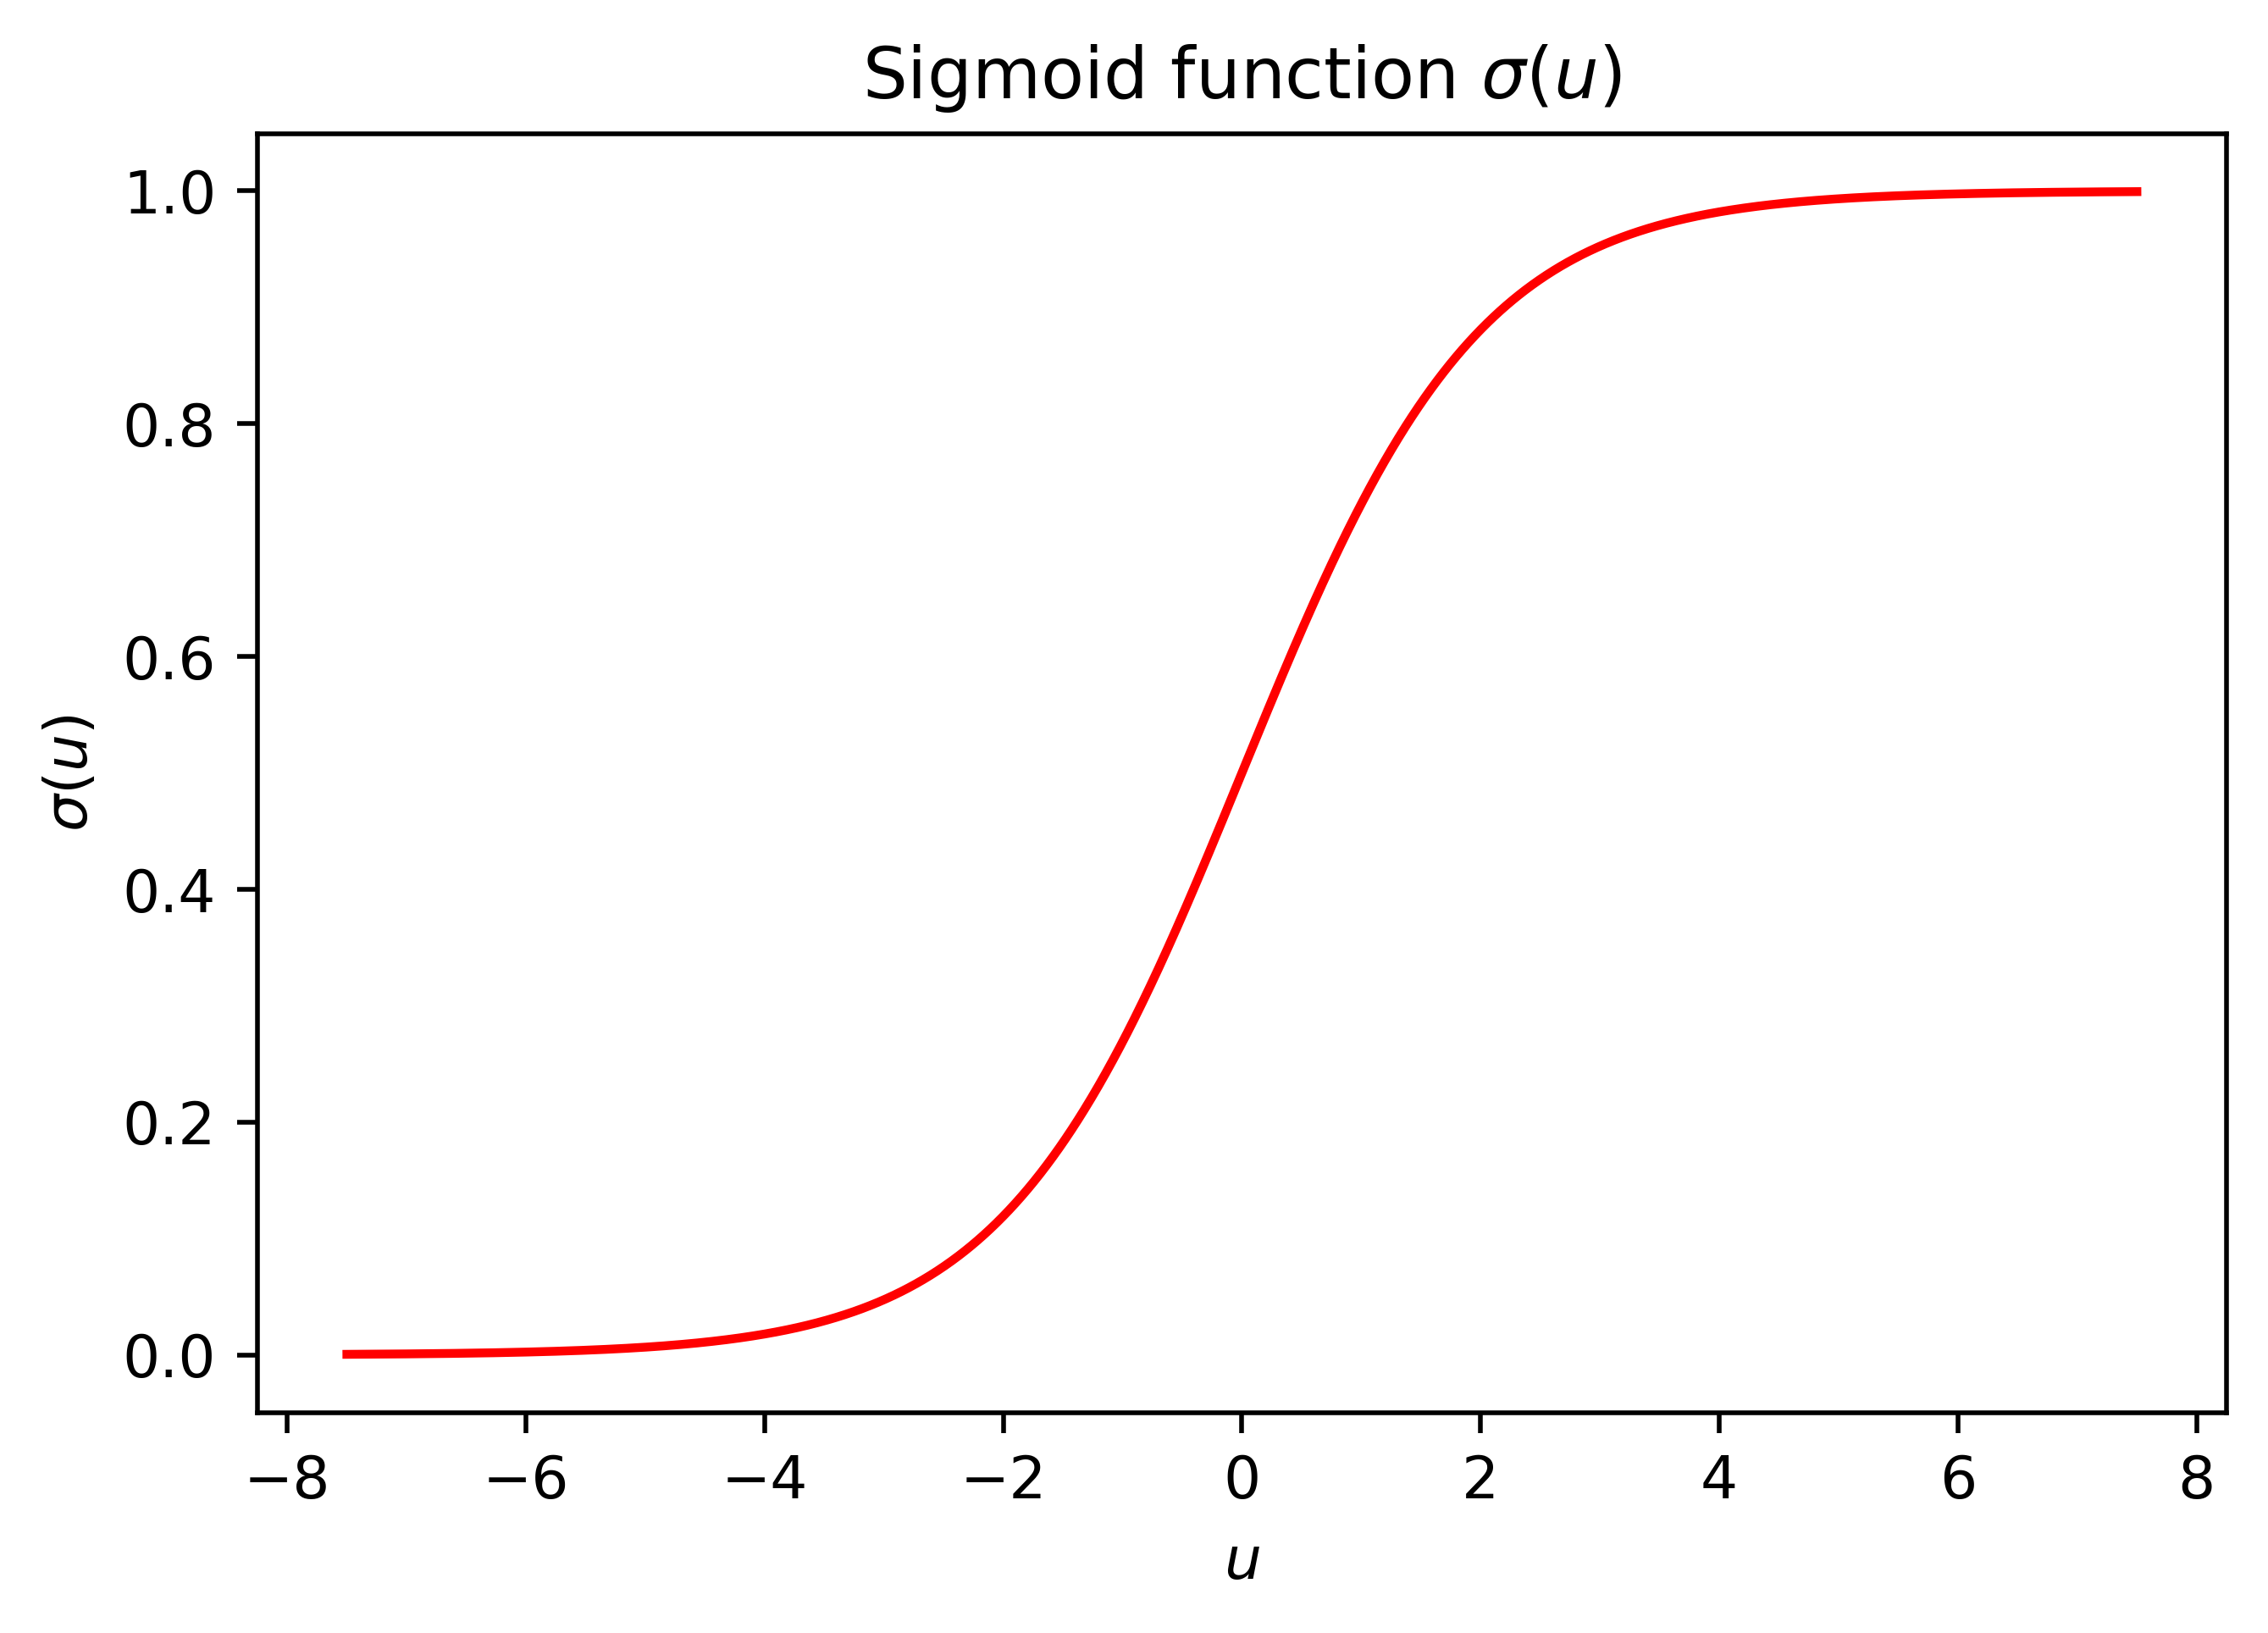
\includegraphics[width=70mm,scale=0.5]{images/classification_images/sigmoid_u.png}
            
            \caption*{$\sigma(u)$ approaches 0 as $u$ approaches $-\infty$, but it never reaches it.}
        \end{figure}
        
        Well, what happens when $u(x)=0$? We get $\sigma(0)=.5$. So, we could use that as our classification: $\sigma(u)>.5$
        
        \begin{figure}[H]
            \centering
            
            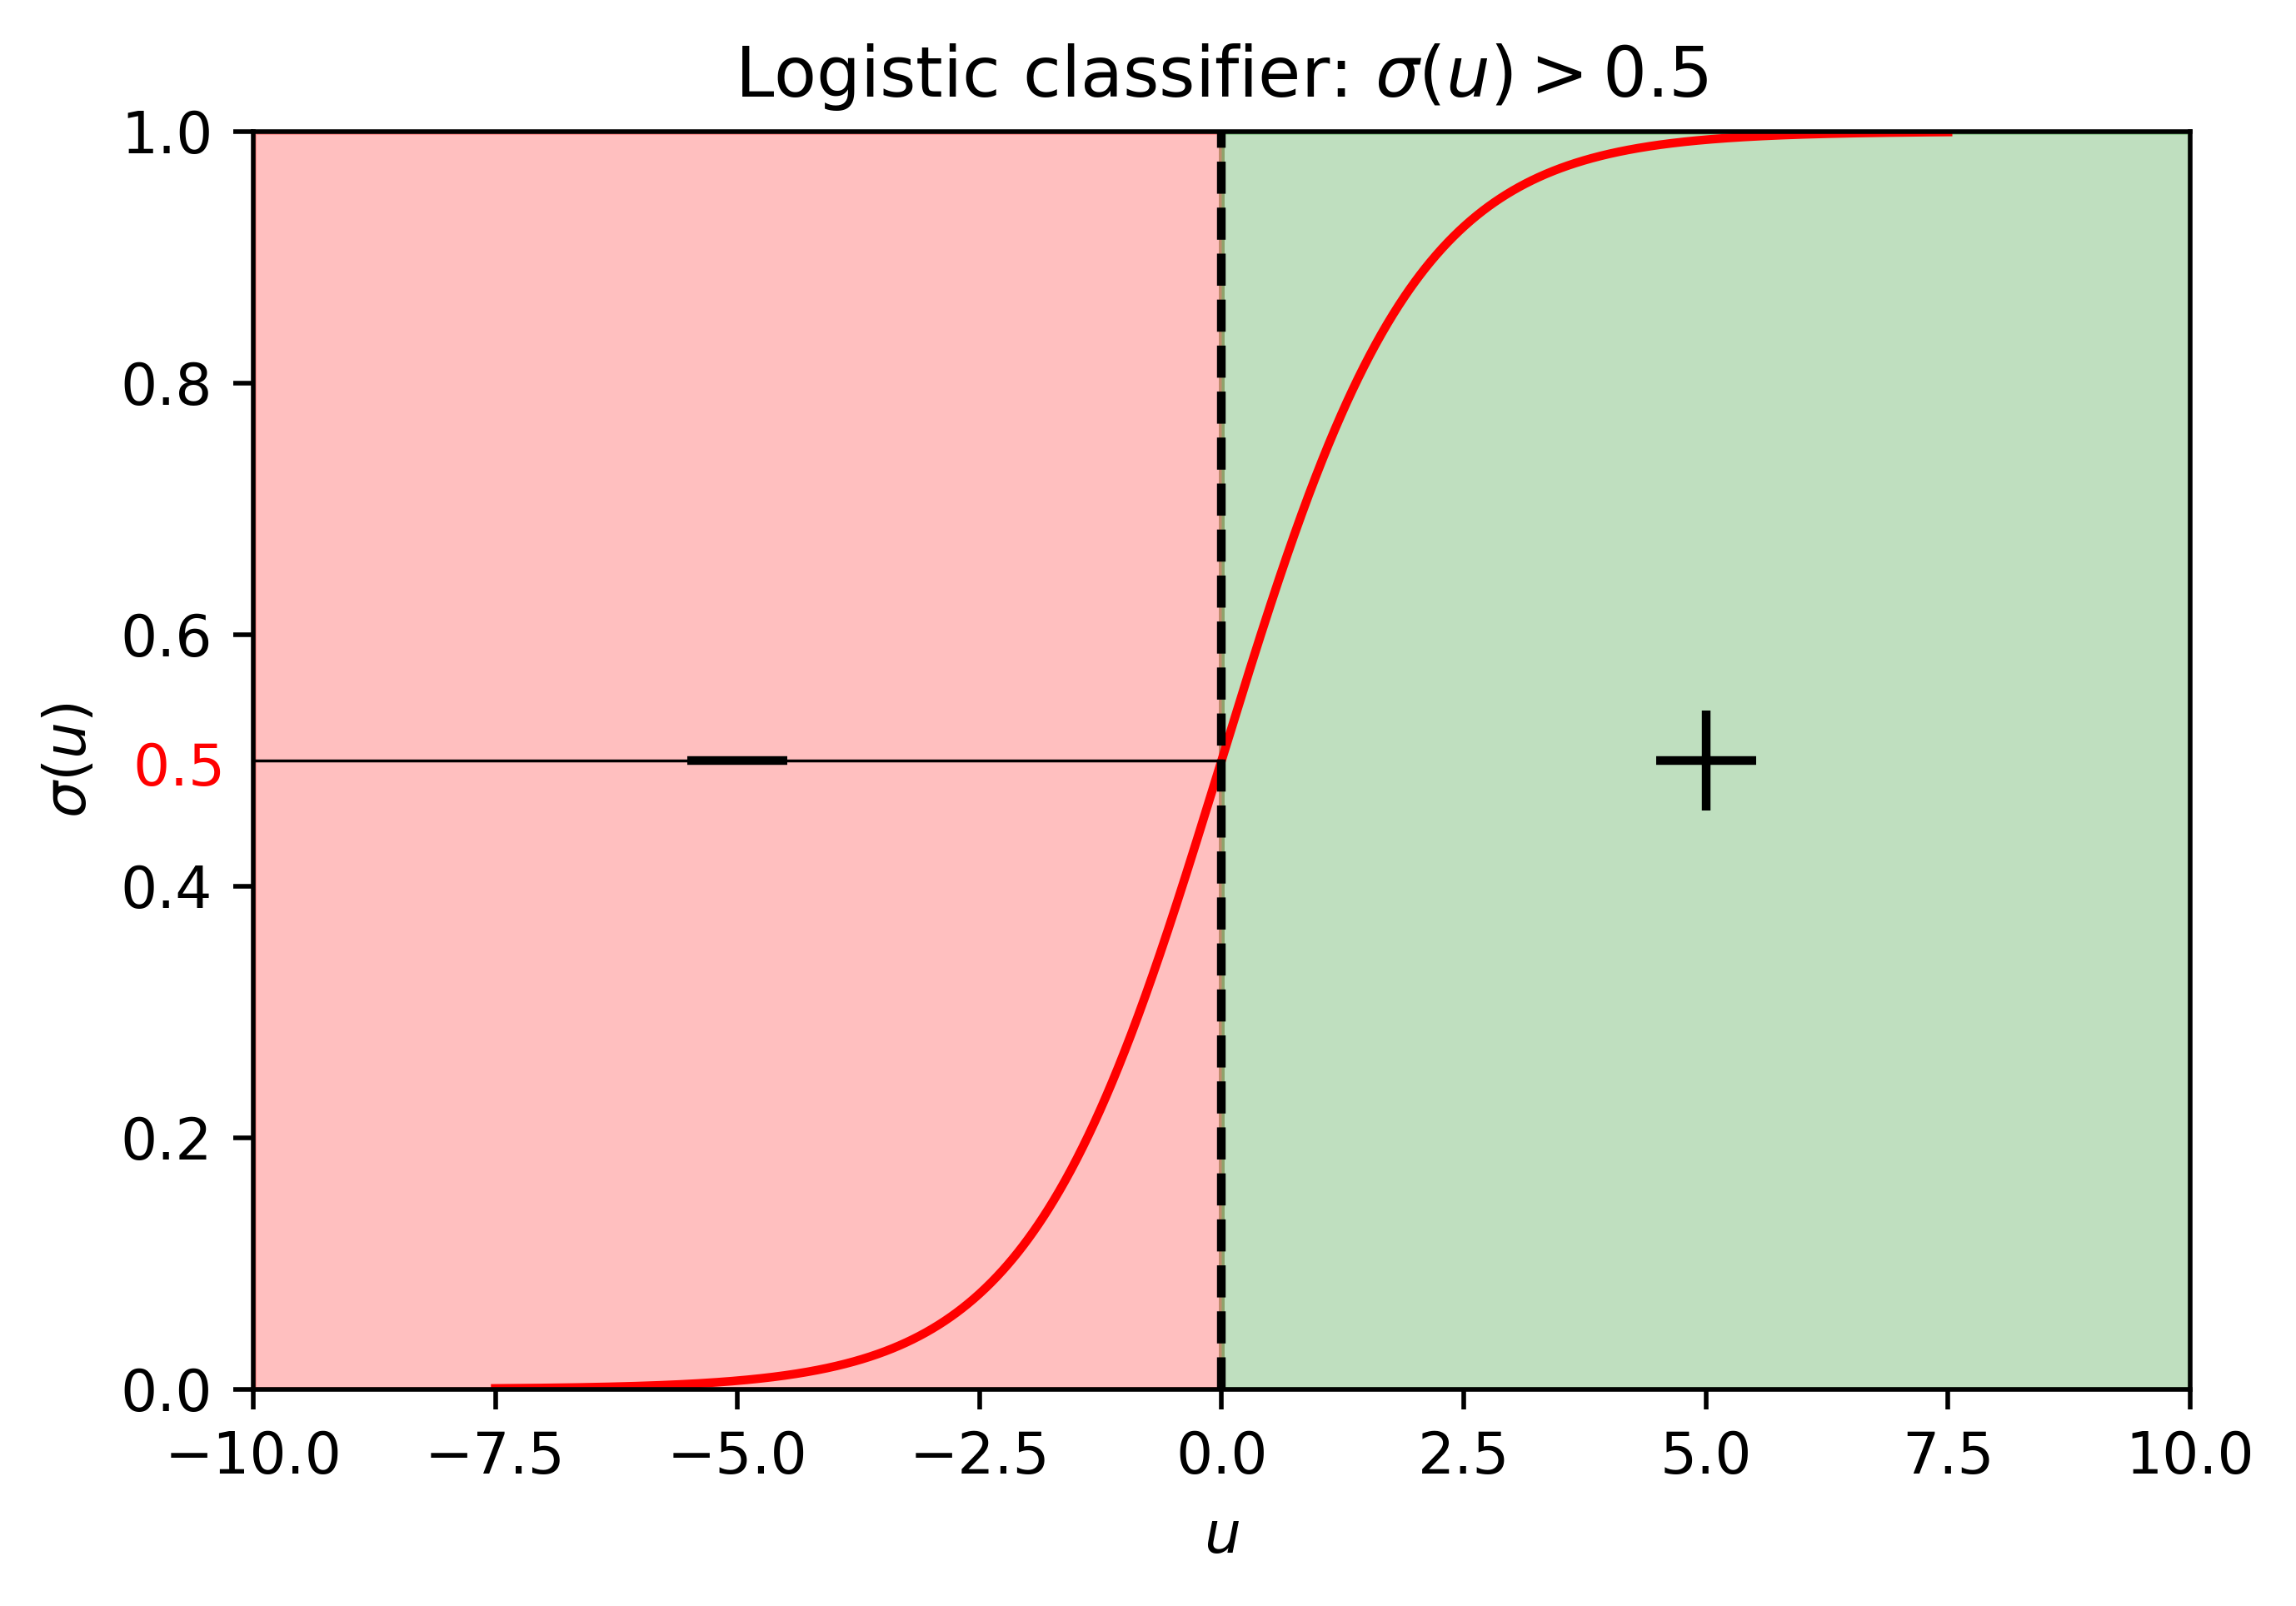
\includegraphics[width=70mm,scale=0.5]{images/classification_images/sigmoid_.5.png}

        \end{figure}
        
        But, we don't necessarily always want to use .5:
        
        \miniex Imagine if you wanted to \textbf{classify} whether someone needs \textbf{life-saving} treatment. Classify $-1$ if sick (they need it), $+1$ if healthy (they don't). 
        
        Let's say you got $\sigma(u)=.6$, so you're only 60\% sure they \textbf{don't} need it. You'd classify that as $\sigma(u)>.5$: they're '\textbf{healthy}'.
        
        Even so, you probably shouldn't \textbf{refuse} someone treatment that's $40\%$ likely to \textbf{save} their life. We might not want to use $\sigma(u)>.5$ after all.
        
        We call the \textbf{boundary} between positive and negative the \textbf{prediction threshold}.\\
        
        \begin{definition}
            The \vocab{prediction threshold} $\sigma_{thresh}$ is the value where you go from \purp{negative} classification to \gren{positive}.
            
            In general, we say
            
            
            
            Our \purp{default} value is a threshold of .5, but our threshold can be \gren{anywhere} in the range
            
            \begin{equation*}
                0 < \sigma_{thresh} < 1
            \end{equation*}
        \end{definition}
        
        \miniex If $\sigma_{thresh}=.9$, we would see:
        
        \begin{figure}[H]
            
            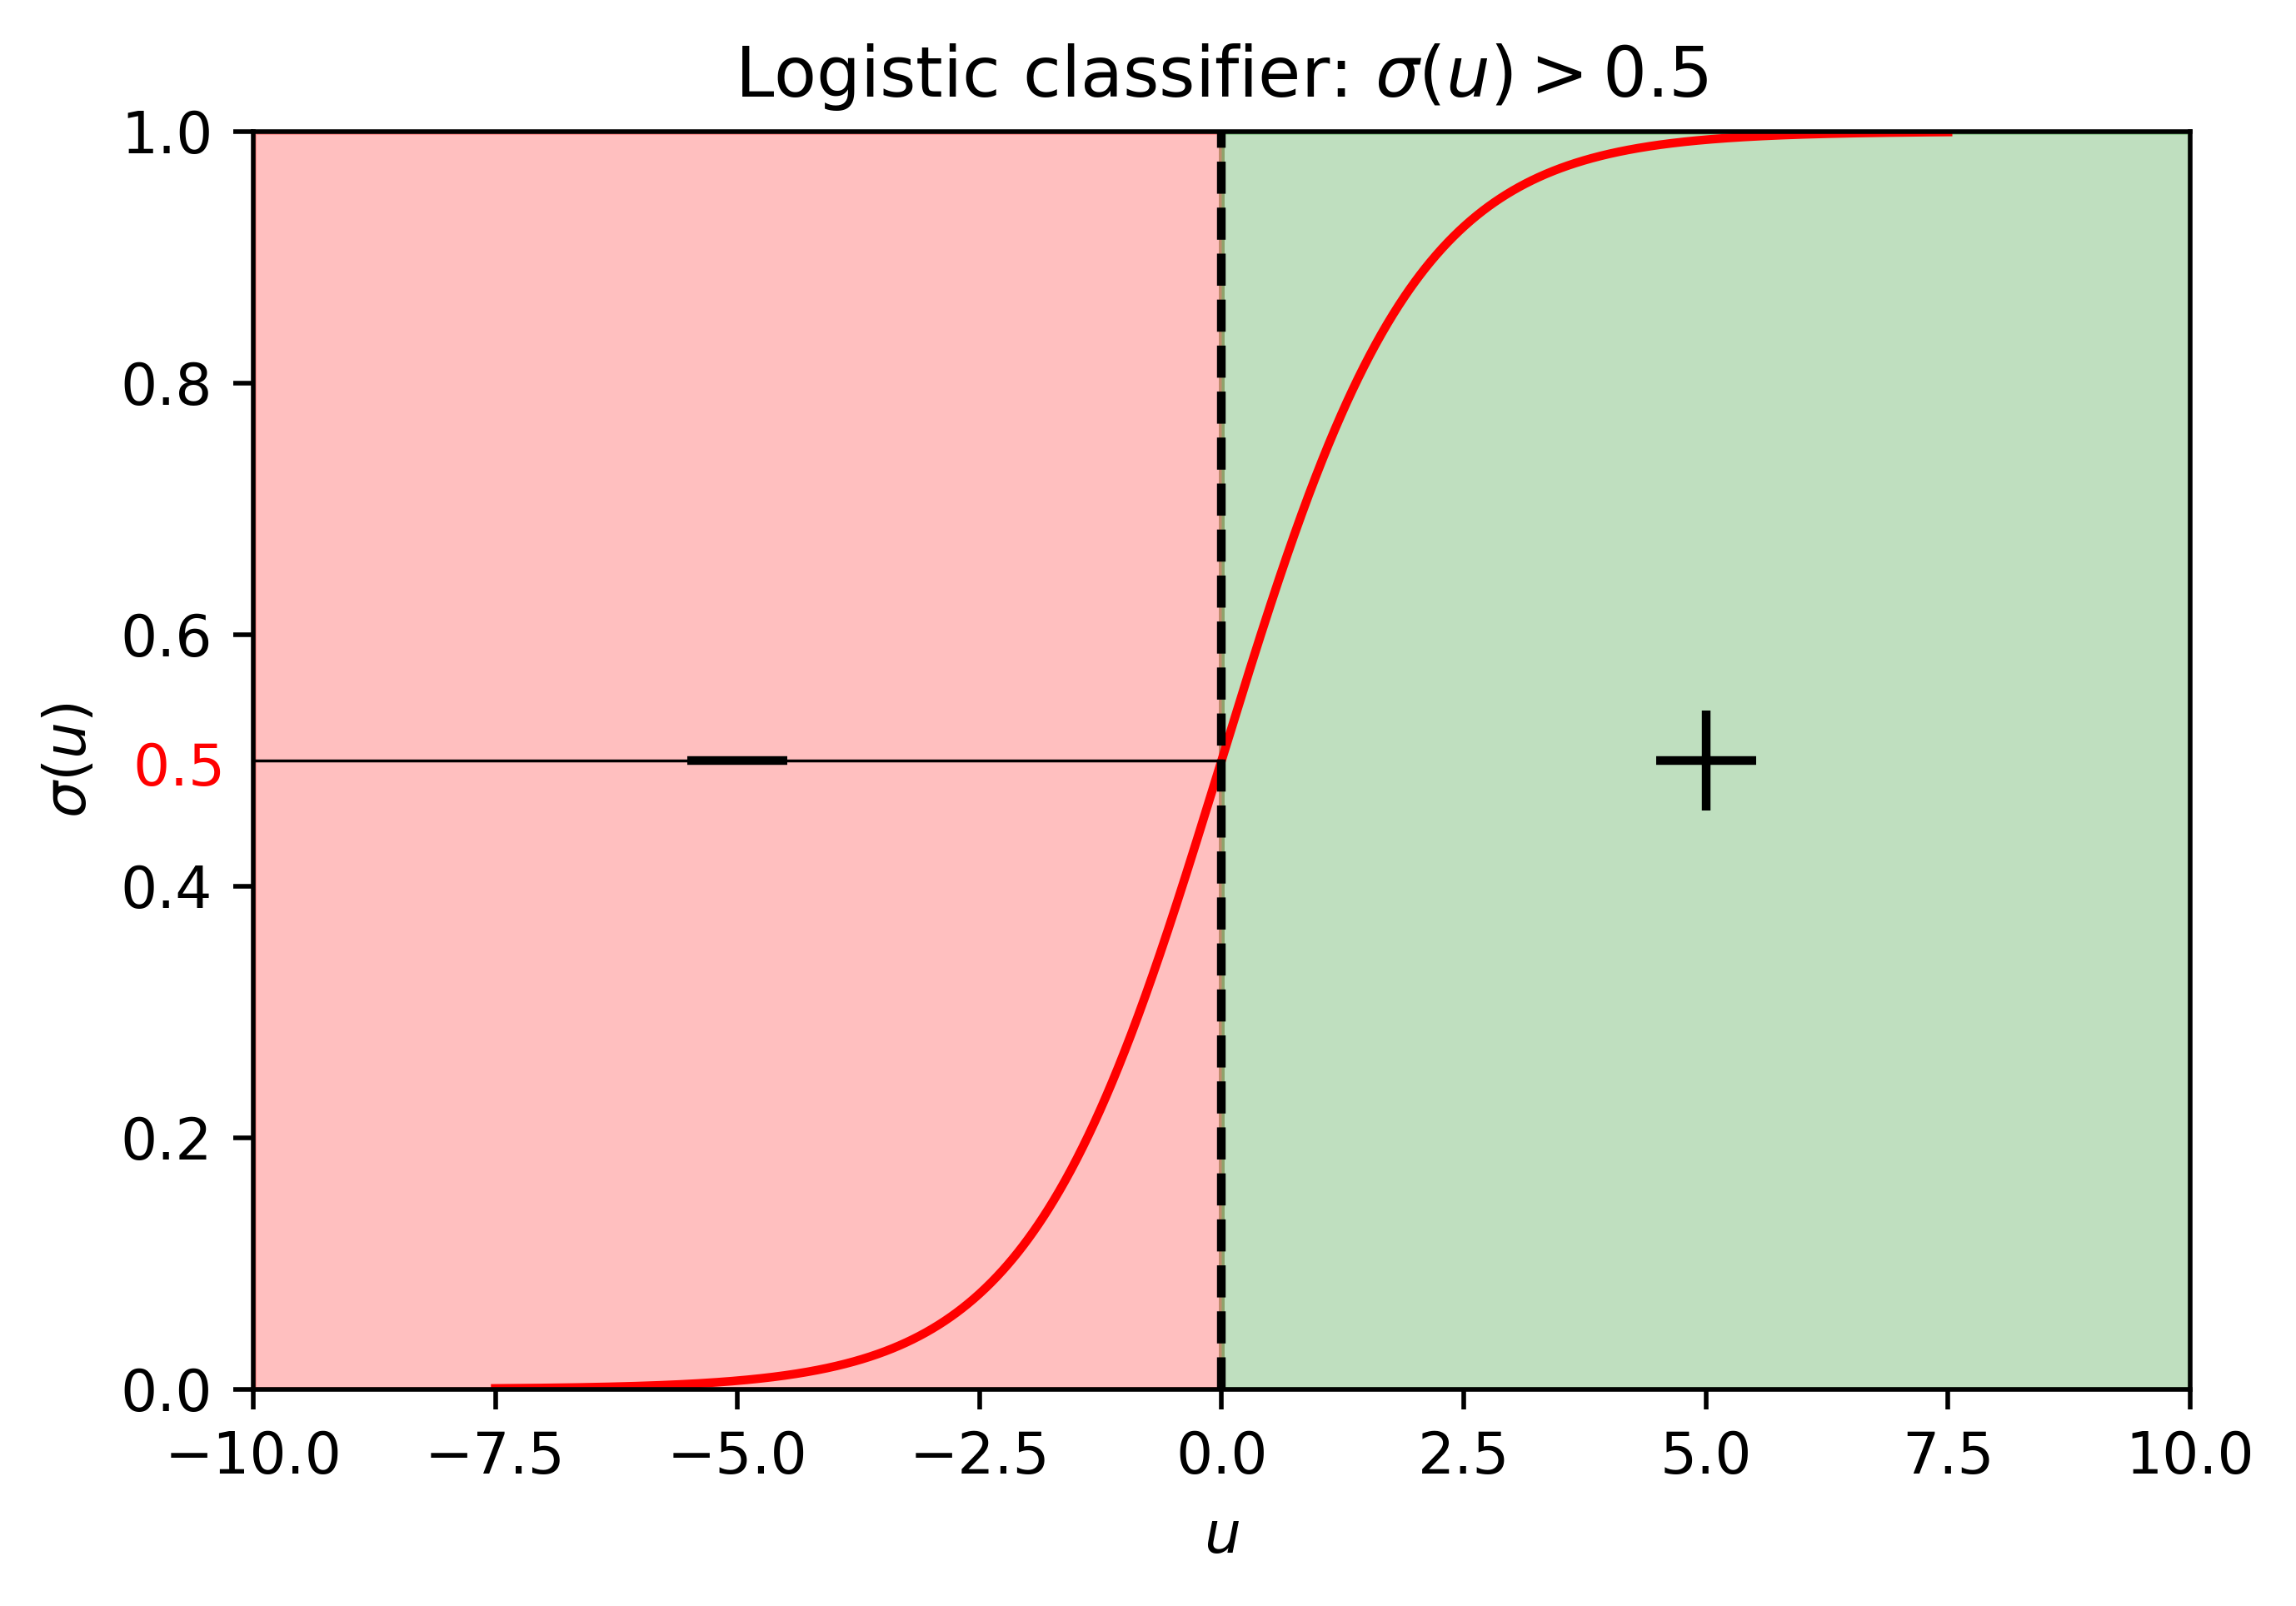
\includegraphics[width=70mm,scale=0.5]{images/classification_images/sigmoid_.5.png}
            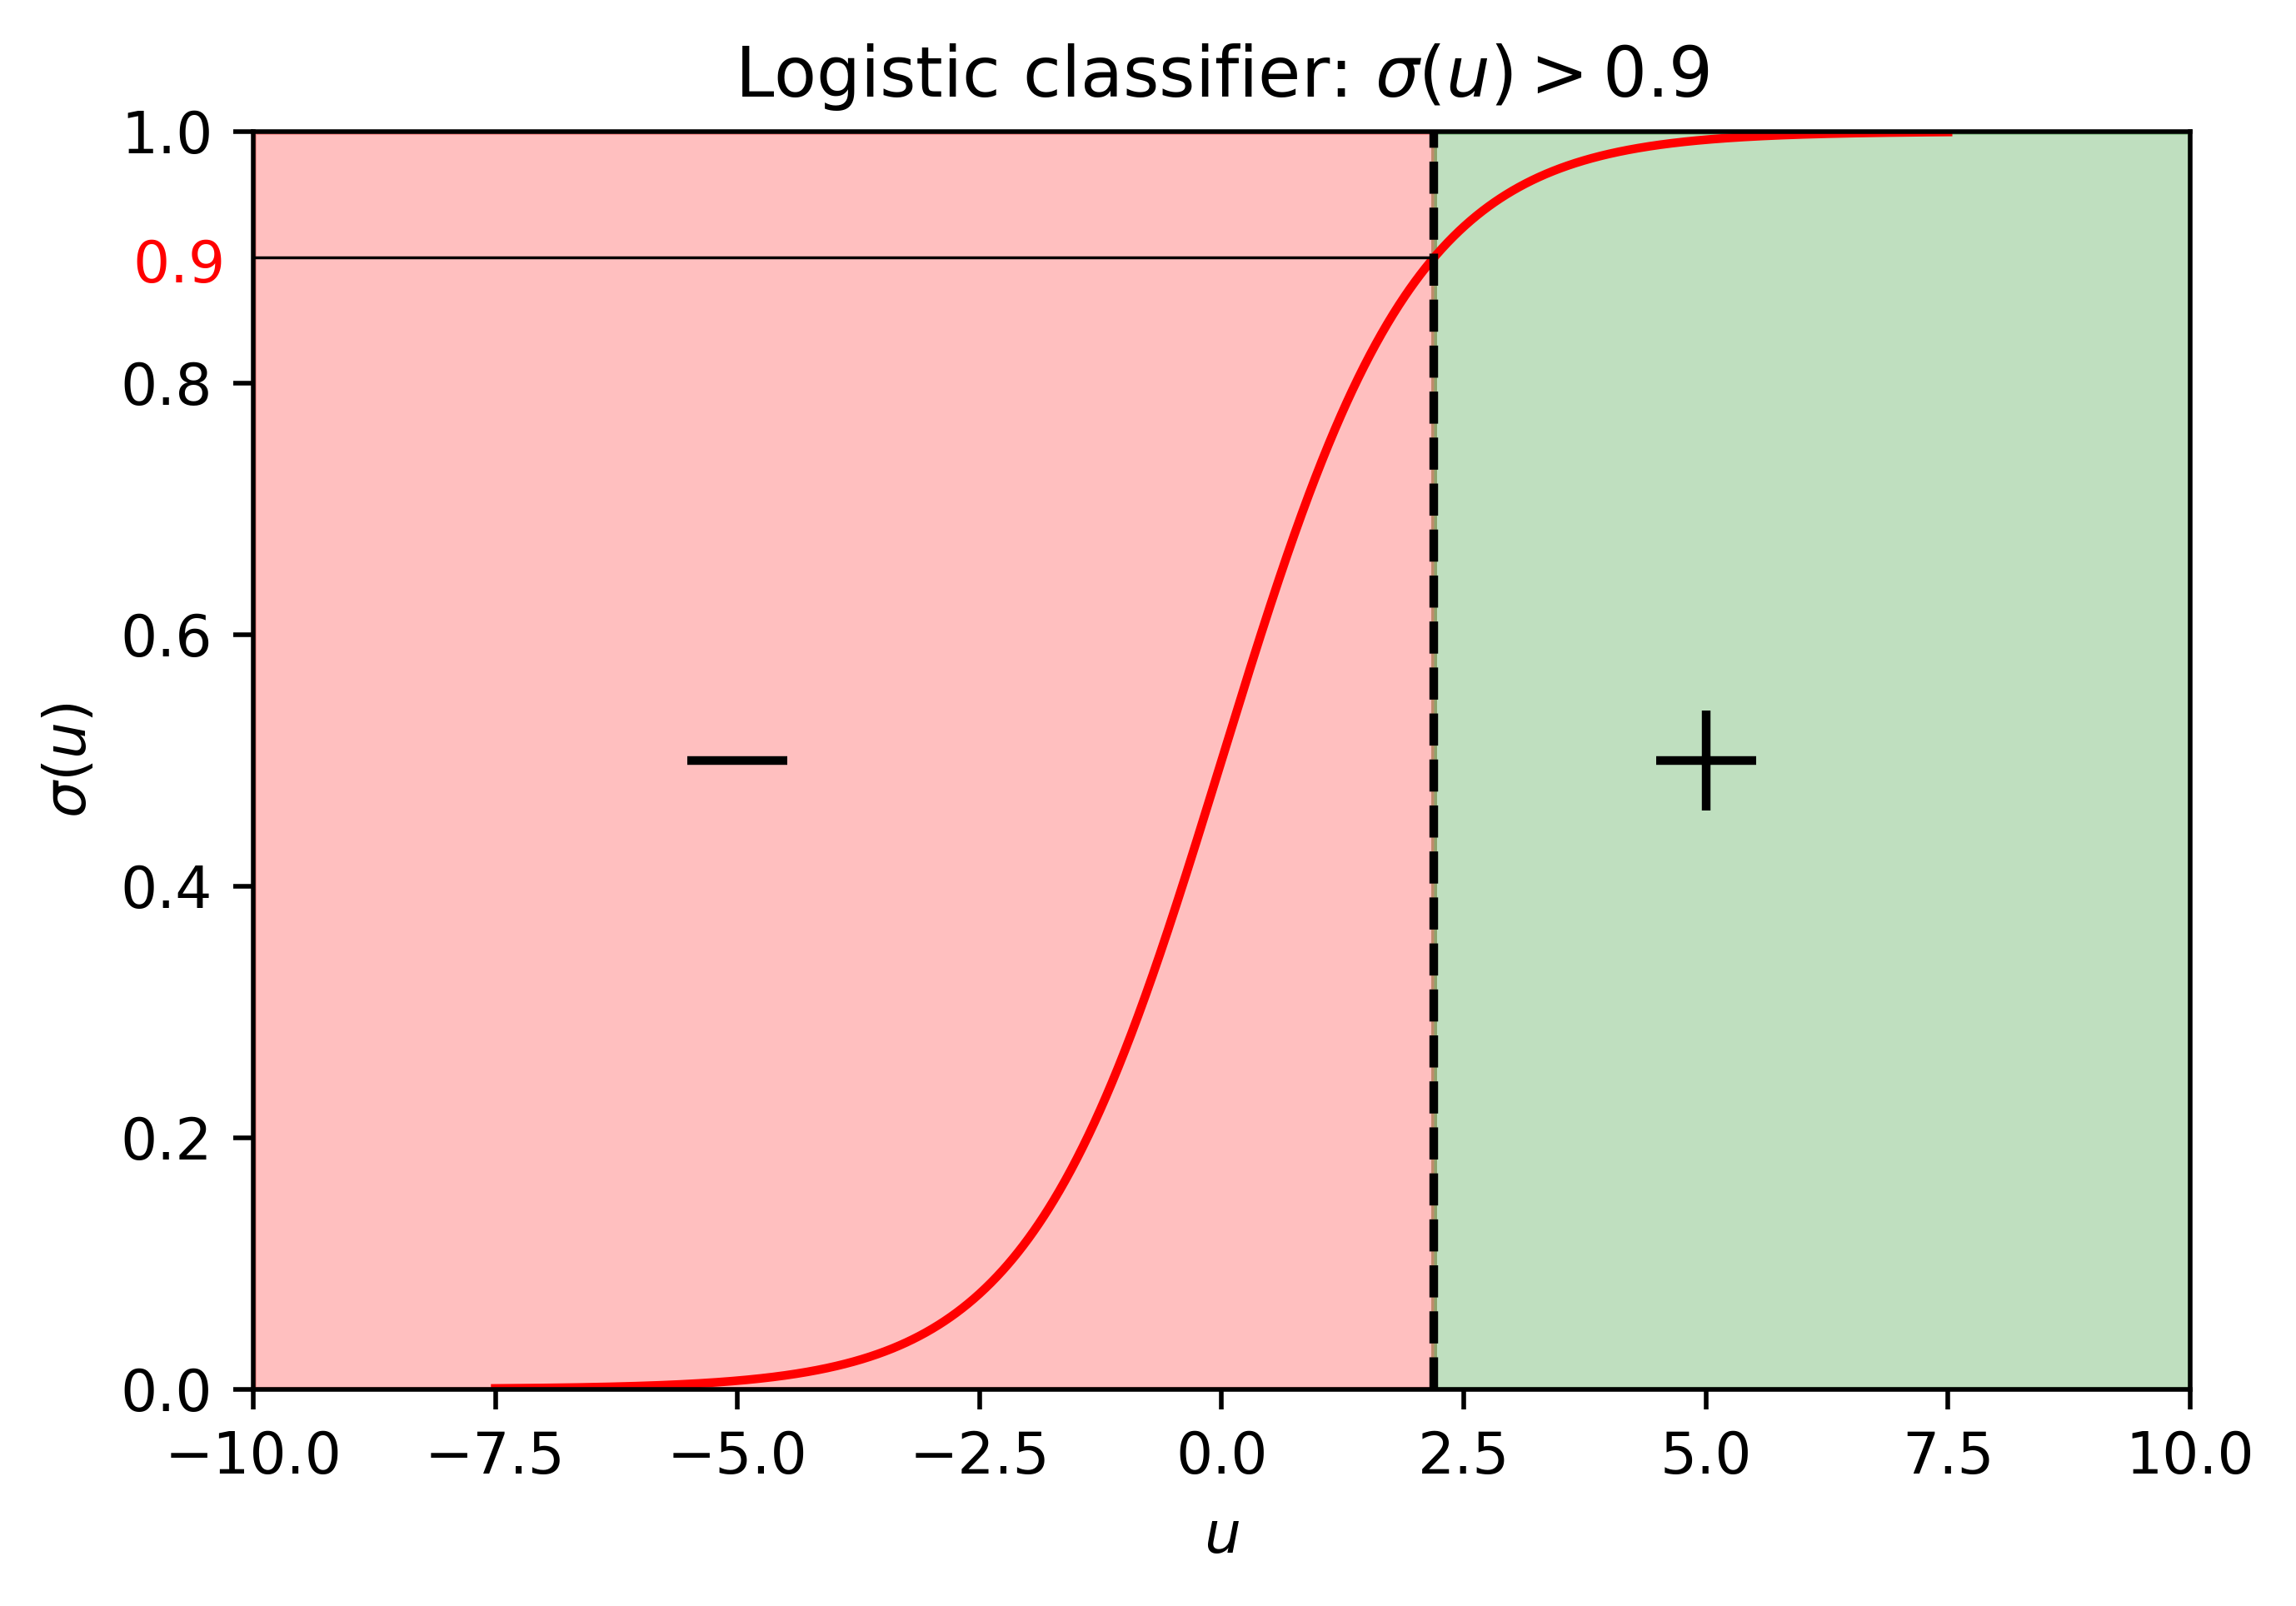
\includegraphics[width=70mm,scale=0.5]{images/classification_images/sigmoid_.9.png}
            \caption*{We switch from a .5 threshold to a .9 threshold.}

        \end{figure}
        
    \subsection*{Linear Logistic Classifier}
        
        This finally gives us our \textbf{linear logistic classifier} (LLC)\\
        
        \begin{kequation}
            The \vocab{linear logistic classifier} is a \purp{binary} classifier of the form
            
            \begin{equation*}
                h(x; \theta) = 
                \begin{cases}
                    +1 & \text{if $\sigma(\red{u(x)})>\sigma_{thresh}$ }\\
                    -1 & \text{otherwise}
                \end{cases}
            \end{equation*}
            
            where 
            
            \begin{equation}
                u=\theta^T x + \theta_0   \qquad\qquad \sigma(u) = \frac{1}{1+e^{-u}}
            \end{equation}
            
            We call it linear because of the linear inner function $u(x)$, and logistic because of the outer function $\sigma(u)$.
        \end{kequation}